% "{'classe':('PSU'),'chapitre':'slci_pi','type':('td'),'titre':'Asservissement par traitement d’image d’une plateforme Hexapode', 'source':' Concours Centrale Supelec PSI 2016','comp':('C1-02','C2-04'),'corrige':True}"
%\setchapterimage{bandeau}
\chapter*{TD \arabic{cptTD} \\ 
Asservissement par traitement d’image d’une plateforme Hexapode -- 
\ifprof Corrigé \else Sujet \fi}
\addcontentsline{toc}{section}{TD \arabic{cptTD} :
Asservissement par traitement d’image d’une plateforme Hexapode -- 
\ifprof Corrigé \else Sujet \fi}

\iflivret \stepcounter{cptTD} \else
\ifprof  \stepcounter{cptTD} \else \fi
\fi

\setcounter{question}{0}
\marginnote{Concours Centrale Supelec PSI 2016.}
\marginnote{\xpComp{COR}{01}\xpComp{COR}{03}}

\begin{marginfigure} [4cm]
\centering
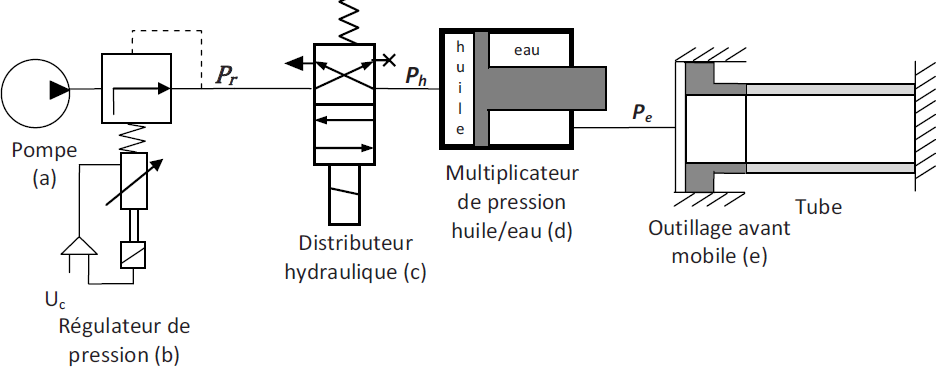
\includegraphics[width=.8\linewidth]{fig_01}
\end{marginfigure}


\section*{Mise en situation}
\ifprof
\else
\begin{obj}
En vue d’asservir la position de la colonne vertébrale à une position de référence, une structure de
commande à partir de l’estimation de la position réelle est mise en place. Après la définition des
modèles nécessaires à la synthèse des lois de commande, l’objet de cette partie est de concevoir le
régulateur de cette architecture de commande.
\end{obj}


Pour la synthèse des régulateurs de la boucle externe, on adopte le modèle du procédé représenté par le schéma-blocs de la figure ci-contre. 

\begin{marginfigure}[3cm]
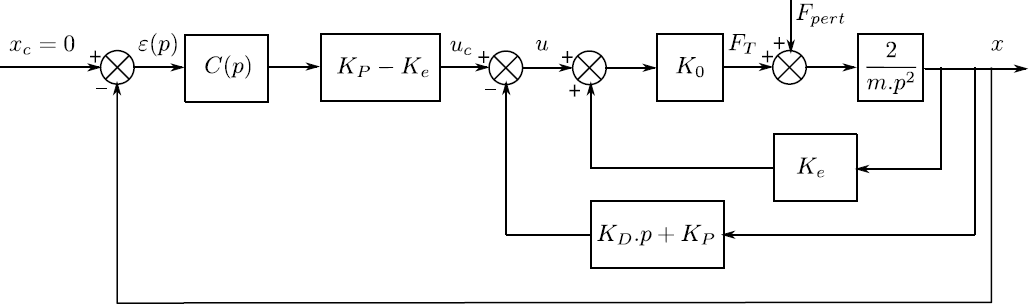
\includegraphics[width=\linewidth]{fig_02}
\caption{Modèle du procédé pour la conception de la loi de commande
de la chaine d’asservissement}
\end{marginfigure}
\fi

\ifprof
\else
\ifcolle
\else
On suppose :
\begin{itemize}
\item qu’une première structure de commande « rapprochée » assure l’asservissement en vitesse des axes et que les caractéristiques dynamiques des six axes asservis sont identiques ;
\item pour un axe donné, que les efforts dus à sa rigidité, à la charge et les couplages avec les autres axes sont modélisés sous la forme d’un signal externe perturbateur unique, ramené en entrée du procédé et dont $F_u(p)$ est la transformée de Laplace ;
\item que les jeux dans les liaisons sont modélisés sous la forme d’un signal perturbateur externe, dont $D(p)$ est la transformée de Laplace, traduisant l’écart de déplacement de la position de l’axe ;
\item pour l’axe considéré que $L^m(p)$, $L^d(p)$ et $L^{de}(p)$ sont respectivement les transformées de Laplace de la position non déformée, de la position de l’axe après déformation et de l’estimation de la position réelle issue de l’évaluation au moyen de l’algorithme de traitement d’images (la grandeur $L^m$ est obtenue au moyen d’une mesure issue d’un capteur placé directement sur l’axe de l’actionneur) ;
\item que $U(p)$ représente la transformée de Laplace de la grandeur de commande (homogène à une tension) de la chaine de motorisation de l’axe considéré.
\end{itemize}
\fi


La chaine de motorisation est modélisée par la fonction de transfert $H(p)=\dfrac{L_m(p)}{U(p)}=\dfrac{0,5}{p\left( 1+0,01 p\right)}$, la chaine d'acquisition et le système de traitement d’images sont modélisés en temps continu comme un retard pur $\tau=\SI{0,04}{s}$.
Pour la chaine d’asservissement, le cahier des charges partiel est le suivant :
%, caractérisé par une pulsation de coupure en boucle ouverte et une marge de phase fixées à priori, est rappelé :
\begin{itemize}
\item pulsation de coupure $\omega_c$ à \SI{0}{dB} en boucle ouverte $\omega_c = \SI{60}{rad.s^{-1}}$;
\item marge de phase $\Delta \varphi \geq 45 \degres$;
\item temps de réponse vis-à-vis de la consigne doit être inférieur à \SI{50}{ms}; 
\item temps de réponse vis-à-vis de la perturbation doit être inférieur à \SI{100}{ms}.
\end{itemize}


\ifcolle
\else
Pour la conception de la loi de commande, il s’agira :
\begin{itemize}
\item de montrer qu’une structure mono-boucle simple ne permet pas d’assurer le cahier des charges partiel ;
\item d’analyser si une structure de commande adaptée aux systèmes à retard peut assurer les performances
escomptées (permettant ainsi de s’affranchir du retard pur de la chaine de mesure par traitement d’images) ;
\item de montrer qu’une structure adaptée aux systèmes à retard complétée par une boucle interne sur la mesure
de position d’un axe non déformé permet de vérifier l’ensemble du cahier des charges.
\end{itemize}

\fi
\fi

\subsection*{Analyse d’une structure mono-boucle}

\ifprof
\else
Une solution simple est d’envisager, dans un premier temps, une structure de commande réalisée directement à
partir de l’estimation $L^{de}(t)$ de la position réelle de l’axe considéré. Cette structure, dont le correcteur est noté
$C_1(p)$ et la consigne $L^{*}(p)$, est représentée par le schéma de la figure suivante.



\begin{figure}[!h]
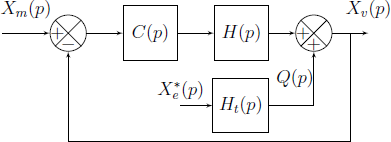
\includegraphics[width=\linewidth]{fig_03}
\caption{Structure de commande à une boucle}
\end{figure}

En raison de la présence de bruits de mesure (signaux non représentés sur les schémas fournis), il n’est pas
souhaitable d’introduire d’action dérivée dans le régulateur de cette boucle. Seuls des correcteurs de type
proportionnel intégral seront envisagés.
\fi

\question{La figure en toute fin de document montre le diagramme de Bode de la fonction $H(p)$. Tracer directement sur cette figure le diagramme de Bode (tracés réels des module et phase) de la fonction de transfert en boucle ouverte non corrigée (soit en prenant $C_1(p)=1$).}

\ifprof
\begin{marginfigure}
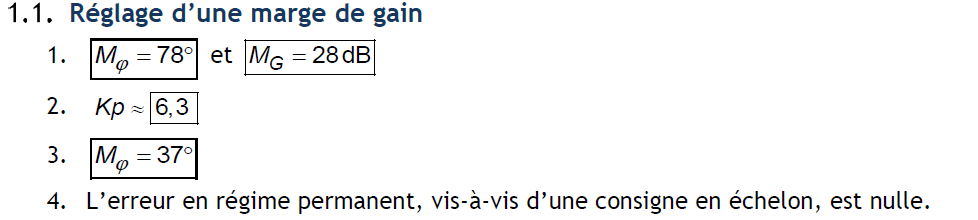
\includegraphics[width=\linewidth]{cor_01}
\caption{FTBO retardée.}
\end{marginfigure}
\begin{corrige}
La fonction de transfert de la FTBO non corrigée est donc $\indice{F}{BO}(p)=H(p)e^{-\tau p}$.

On note $\indice{G}{dB}(\omega)$ le gain de la fonction de transfert et $\varphi(\omega)$ la phase. 
 
$e^{-\tau j \omega}$ est un nombre complexe de gain 1 et de phase $-\tau\omega = -0,04 \omega $ (en rad). 
En degrés, le retard ajoute un déphasage de  $-0,04 \omega \dfrac{180}{\pi}$. 
Ainsi :
\begin{itemize}
\item pour $\omega = \SI{1}{rad/s}$, la phase est baissée de 2\degres,
\item pour $\omega = \SI{10}{rad/s}$, la phase est baissée de 20\degres,
\item pour $\omega = \SI{50}{rad/s}$, la phase est baissée de 100\degres,
\item pour $\omega = \SI{100}{rad/s}$, la phase est baissée de 220\degres ...
\end{itemize}
Ce qui permet de modifier le diagramme de bode de la phase. 

\end{corrige}
\else
\fi


\question{Au regard des tracés de la question précédente et des performances souhaitées par le cahier des charges :
\begin{itemize}
\item compte tenu de la pulsation de coupure et de la marge de phase souhaitées, déterminer les deux contraintes (sur le module et l’argument) que le correcteur $C_1(j\omega)$ doit vérifier pour les deux cas : procédé sans retard pur et procédé avec la présence du retard pur $\tau$;
\item en argumentant la réponse à l’aide du tracé des allures des diagrammes de Bode (directement sur la copie) d’un correcteur de type proportionnel intégral $C_1(p) = K_1\left(1 +
\dfrac{1}{T_{i1}p}\right)$, justifier qu’un correcteur de ce type :
\begin{itemize}
\item ne permet pas d’atteindre les performances exigées en présence du retard de mesure ;
\item peut être toutefois envisagé en absence du retard dans la chaine de mesure.
\end{itemize}
\end{itemize}}


\ifprof
\begin{corrige}
D'après le cahier des charges : 
\begin{itemize}
\item pulsation de coupure $\omega_c$ à \SI{0}{dB} en boucle ouverte $\omega_c = \SI{60}{rad.s^{-1}}$;
\item marge de phase $\Delta \varphi \geq 45 \degres$.
\end{itemize}

Pour le système non retardé, le correcteur PI permettra de remonter le gain de $\SI{45}{dB}$ afin d'obtenir la pulsation de coupire souhaitée. En réglant $T_i$ tel que $1/T_i = 60/10$, on pourra conserver une marge de phase de 55 à 60\degres ce qui est compatible avec le cahier des charges (ou la descebdre à 45\degres en affinant la valeur de $T_i$.


Pour le systèmer retardé, le correcteur PI permettra de régler la pulsation de coupure, mais la phase est trop basse pour espérer la corriger ainsi.  
\end{corrige}
\else
\fi


\subsection*{Structure de commande adaptée à un système avec retard}

\ifprof
\else
Pour remédier au problème mis en évidence à la question précédente, il est envisagé d’utiliser une structure de commande
adaptée aux systèmes comportant des retards. La figure suivante montre deux structures de commande correspondant
d’une part au schéma réel (a) représentant la réalisation de la commande ($X(p)$ est la transformée de Laplace
d’une grandeur $x(t)$ interne au régulateur), d’autre part un schéma fictif (b).

\begin{figure}[!h]
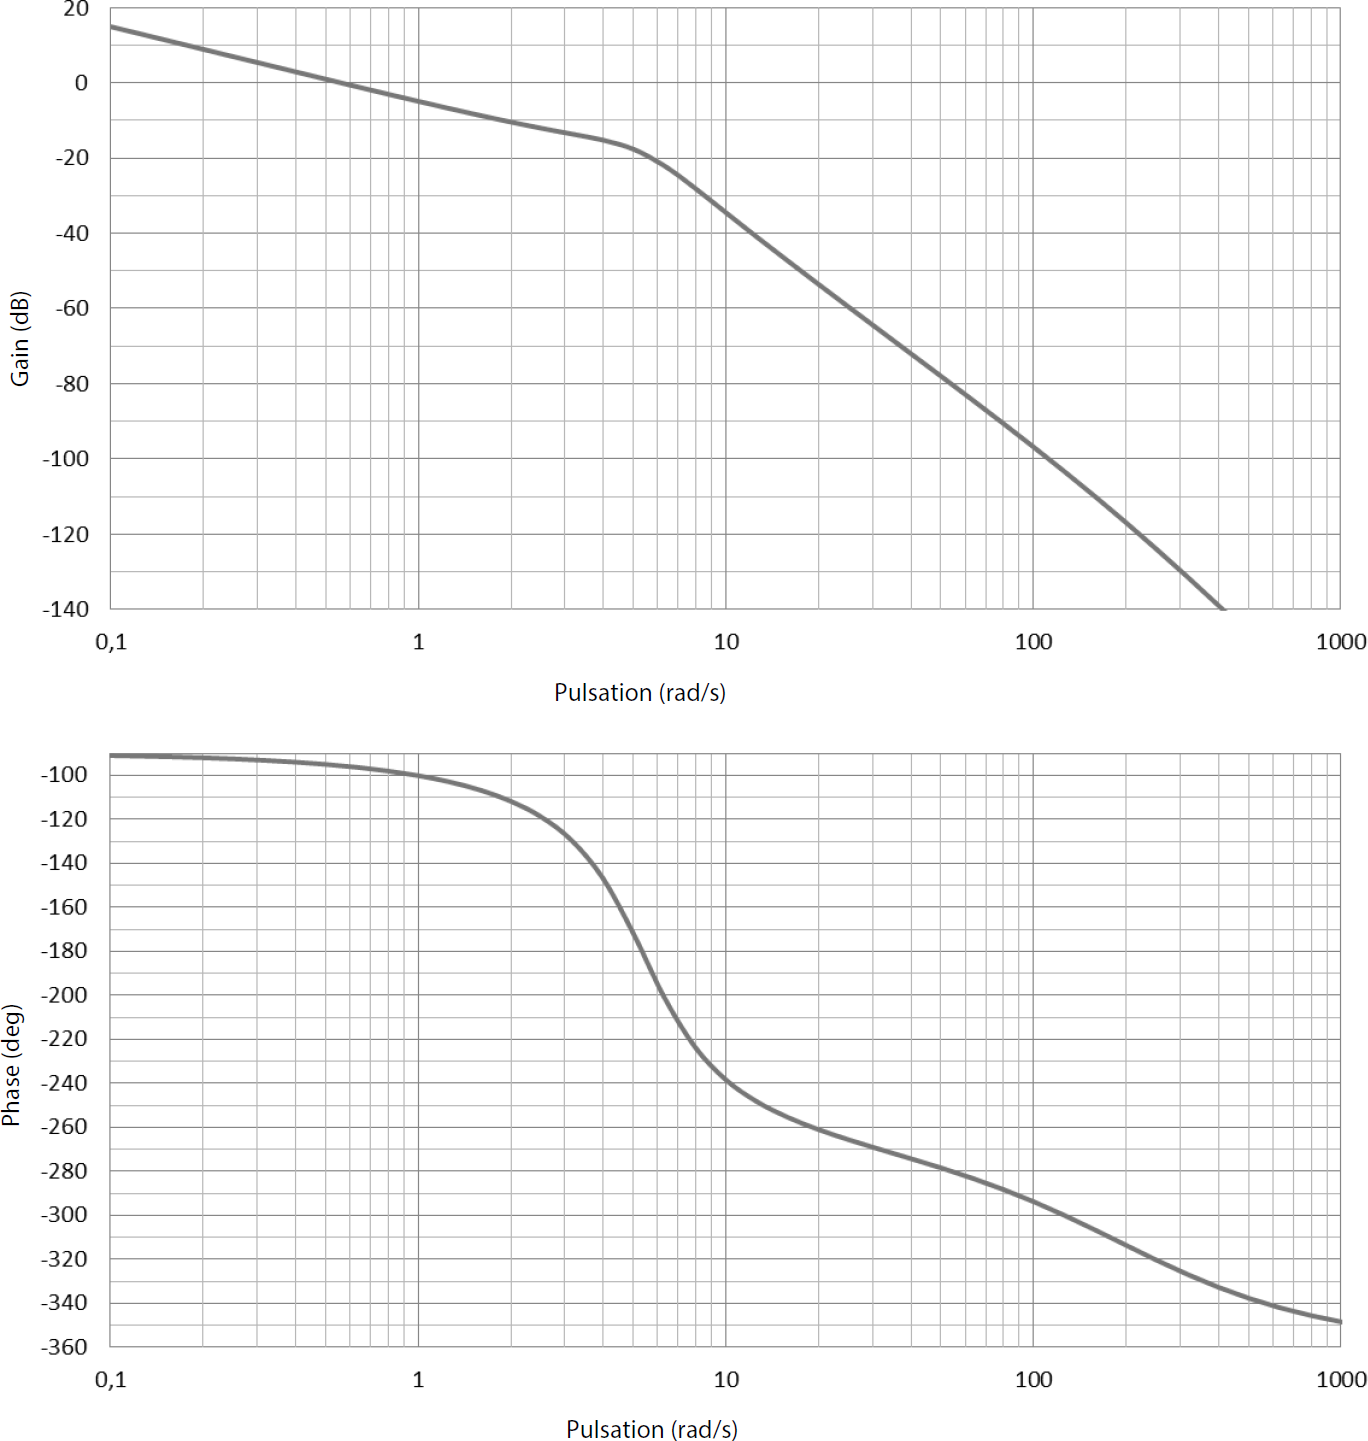
\includegraphics[width=\linewidth]{fig_04}
\caption{Structure de commande adaptée aux systèmes à retard}
\end{figure}
\fi

\question{En utilisant le schéma fictif (b) et le diagramme de Bode de la figure B du document réponse, déterminer le
correcteur de type proportionnel intégral $C(p)= K\left( 1+\dfrac{1}{T_ip}\right)$ permettant d’assurer les performances exprimées
par le cahier des charges partiel. Pour concevoir ce régulateur, la démarche suivante pourra être suivie :
\begin{itemize}
\item déterminer la condition en phase, soit $\arg(C(j\omega))$, que doit vérifier le correcteur au regard de la marge de
phase souhaitée. En déduire alors la valeur numérique du temps d’action intégrale $T_i$ ;
\item pour la valeur de $T_i$ obtenue, déterminer alors la valeur du gain $K$ permettant d’assurer le cahier des charges partiel.
\end{itemize}}

\ifprof
\begin{corrige}
Le système non corrigé a une marge de phase de $60\degres$. On veut que la pulsation de coupure soit de 
$\SI{60}{rad/s}$.

On cherche donc $T_i$, tel que $\text{arg}\left( K\dfrac{T_i p+1}{T_i p }\right) =-15\degres$ pour 
$\SI{60}{rad/s}$.
Soit $\arctan \left(60 T_i\right)- 90 = -15$ soit $T_i = \dfrac{\tan 75}{60} \simeq \SI{0,062}{s}$.

De plus pour que la pulsation de coupure soit à $\SI{60}{rad/s}$, il faut que $\left| K\dfrac{T_i p+1}{T_i p }\right| = 10^{\dfrac{45}{20}} $ pour $\SI{60}{rad/s}$.

On a donc $K \sqrt{T_i^2 \omega ^2 + 1 } = 60 T_i\times  10^{\dfrac{45}{20}}$ et $K =  \dfrac{0,062\times 60\times  10^{\dfrac{45}{20}} }{\sqrt{0,062^2 \times 60^2 + 1 }} = 171$.
\end{corrige}
\else
\fi


\question{
Pour une consigne nulle $L^*(t)$, une perturbation en sortie nulle $d(t)=0$ et un échelon de perturbation en entrée $f_u(t)=F_0 h(t)$ où h(t) est l’échelon d’Heaviside :
\begin{itemize}
\item déterminer la valeur en régime permanent de la grandeur de commande $\lim\limits_{t \to \infty} u(t)$ (ce calcul sera effectué en utilisant la structure de la figure 3(a)) ;
\item compte tenu de la forme de $H(p)$, en déduire alors le comportement de la grandeur $x(t)$ lorsque $t$ tend vers l’infini ;
\item au regard de ce comportement, discuter alors des performances de cette structure de commande et conclure quant à sa pertinence sur l’asservissement de l’Hexapode.
\end{itemize}
}

\ifprof
\begin{corrige} 
Pour le schéma $a$, on a 
$U(p) =-L^d(p) e^{-\tau p} \times \dfrac{C(p)}{1+C(p)H(p)\left( 1- e^{\tau p}\right)}$ 
et $L^d(p) = H(p)\left( U(p)+F_u(p)\right)$.
On a donc 
$U(p) =-H(p)\left( U(p)+F_u(p)\right) e^{-\tau p} \times \dfrac{C(p)}{1+C(p)H(p)\left( 1- e^{\tau p}\right)}$ .

$\Rightarrow 
U(p) \left(1+  \dfrac{C(p) H(p)e^{-\tau p} }{1+C(p)H(p)\left( 1- e^{\tau p}\right)} \right)=-\dfrac{C(p) H(p) F(p) e^{-\tau p} }{1+C(p)H(p)\left( 1- e^{\tau p}\right)}$

$\Rightarrow 
U(p)   \dfrac{1+C(p)H(p)\left( 1- e^{\tau p}\right)+C(p) H(p)e^{-\tau p} }{1+C(p)H(p)\left( 1- e^{\tau p}\right)} =-\dfrac{C(p) H(p) F(p) e^{-\tau p} }{1+C(p)H(p)\left( 1- e^{\tau p}\right)}$

$\Rightarrow 
U(p)   =-\dfrac{C(p) H(p) F(p) e^{-\tau p} }{1+C(p)H(p)\left( 1- e^{\tau p}\right)+C(p) H(p)e^{-\tau p}}$


$\Rightarrow 
U(p)   =-\dfrac{C(p) H(p) F(p) e^{-\tau p} }{1+C(p)H(p)}$


On a alors, 
$\lim\limits_{t \to \infty} u(t) = \lim\limits_{p \to 0} - p \dfrac{C(p) H(p) F(p) e^{-\tau p} }{1+C(p)H(p)}$

$= \lim\limits_{p \to 0}  -\dfrac{K\dfrac{1+T_i p}{T_i p} \dfrac{0,5}{p\left(1+0,01 p \right)} F_0 e^{-\tau p} }{1+K\dfrac{1+T_i p}{T_i p}\dfrac{0,5}{p\left(1+0,01 p \right)}}$
$= \lim\limits_{p \to 0} - \dfrac{0,5K\left(1+T_i p\right)  F_0 e^{-\tau p} }{T_i p^2\left(1+0,01 p \right) +0,5K\left(1+T_i p\right)}$
$=  -  F_0$

Le signal de commande sera ensuite intégré par la fonction de transfert $H(p)$. $X(p)$ divergera donc. 
La commande n'est donc pas stable.

\end{corrige}
\else
\fi

\subsection*{Analyse d’une structure de commande à deux boucles}
\ifprof
\else
Pour remédier au problème mis en évidence à la question précédente, il est envisagé une structure à deux boucles définies ainsi :
\begin{itemize}
\item une boucle interne réalisée à partir de la mesure de la position non déformée de l’axe $L^m(t)$ permet d’asservir cette grandeur à une consigne de référence $L^{m*}(t)$. Le calcul du correcteur de la boucle interne est hors du cadre de cette étude, et on note $T(p)=\dfrac{L^m(p)}{L^{m*}(p)}$ la fonction de transfert en boucle fermée de la boucle
interne ;
\item la boucle externe, réalisée à partir de la grandeur estimée $L^{de}(t)$.
\end{itemize}
La nouvelle structure de commande est représentée par le schéma de la figure suivante où la représentation de la
boucle interne est limitée à sa fonction de transfert en boucle fermée $T(p)$ où :
\begin{itemize}
\item $T(p) = \dfrac{L^m(p)}{L^{m*}(p)}= \dfrac{1}{\left(1+0,05p\right)^2}$ est la fonction de transfert en boucle fermée de l’asservissement de position de l’axe non déformée (elle est ainsi la fonction de transfert de la boucle interne non représentée sur la figure) ;
\item $L^{m*}(p)$ est la consigne de l’asservissement de la boucle interne ;
\item l’effet de la perturbation $F_u(p)$ est réduit par la boucle interne, et son influence peut être négligée;
\item les seules perturbations se limitent alors à celles dues aux jeux, soit le signal de transformée de Laplace $D(p)$.
\end{itemize}
Pour la conception de la loi de commande :
\begin{itemize}
\item une approche identique à celle de la partie précédente adaptée au cas des systèmes présentant des retards est utilisée ;
\item on synthétise dans ce cas un correcteur $C_2(p) = K_2 \left( 1+\dfrac{1}{T_{i2}p}\right) $ de type PI sans prendre en compte le retard et le régulateur $R_e(p)$ est réalisé en utilisant $C_2(p)$ selon une structure identique à celle de la figure précédente (a) ;
\item le calcul du régulateur $C_2(p)$ ne fait pas partie de cette étude, on suppose cependant qu’il permet d’assurer les exigences du cahier des charges.
\end{itemize}


\begin{figure}[!h]
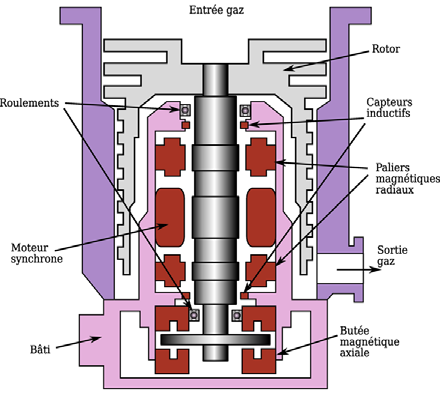
\includegraphics[width=\linewidth]{fig_05}
\caption{Modèle de commande avec une boucle interne intégrée}
\end{figure}
\fi


\question{En utilisant la même démarche que celle de la question précédente, déterminer la valeur de la grandeur $L^{m}(t)$ en régime permanent, soit 
$\lim\limits_{t\to\infty} L^{m*}(t)$, en réponse à une perturbation $d(t)$ en échelon $d(t)=D_0 h(t)$. Au regard des différents éléments constitutifs de la boucle de régulation, justifier qualitativement que la réalisation du régulateur $R_e(p)$ selon le schéma de la figure 3(a) reste stable du point vue interne.}

\ifprof
\begin{corrige}
On a $L^m(p)=-L^d(p) e^{-\tau p} \dfrac{C_2(p)}{1+C_2(p)\left(1-e^{-\tau p}\right)T(p)} T(p)$ 
et $L^d(p)=L^m(p)+D(p)$.
Ainsi,
$L^m(p)=-\left( L^m(p)+D(p)\right) e^{-\tau p} \dfrac{C_2(p)}{1+C_2(p)\left(1-e^{-\tau p}\right)T(p)} T(p)$ 

$\Rightarrow L^m(p)\left(1+ \dfrac{C_2(p) T(p)e^{-\tau p}}{1+C_2(p)\left(1-e^{-\tau p}\right)T(p)}  \right)=- \dfrac{C_2(p) D(p) T(p)e^{-\tau p}}{1+C_2(p)\left(1-e^{-\tau p}\right)T(p)} $

$\Rightarrow L^m(p)\left(1+C_2(p)\left(1-e^{-\tau p}\right)T(p)+ C_2(p) T(p)e^{-\tau p}  \right)=- C_2(p) D(p) T(p)e^{-\tau p}$ 


$\Rightarrow L^m(p)=- \dfrac{C_2(p) D(p) T(p)e^{-\tau p}}{1+C_2(p)T(p) }$ 

On a donc $L^m(p)=- \dfrac{K_2 \left( 1+\dfrac{1}{T_{i2}p}\right)  \dfrac{1}{\left(1+0,05p\right)^2}e^{-\tau p}}{1+K_2 \left( 1+\dfrac{1}{T_{i2}p}\right)\dfrac{1}{\left(1+0,05p\right)^2}}D(p)$

$=- \dfrac{K_2 \dfrac{T_{i2}p+1}{T_{i2}p}  \dfrac{1}{\left(1+0,05p\right)^2}e^{-\tau p}}{1+K_2 \dfrac{T_{i2}p+1}{T_{i2}p}\dfrac{1}{\left(1+0,05p\right)^2}}D(p)$
$=- \dfrac{K_2 \left(T_{i2}p+1\right)  e^{-\tau p}}{T_{i2}p\left(1+0,05p\right)^2+K_2 \left(T_{i2}p+1\right)}D(p)$

On a alors, 
$\lim\limits_{t \to \infty} L^m(t) = \lim\limits_{p \to 0} p L^m(p)  $ 
$ =-D_0  \dfrac{K_2 }{K_2} =-D_0$.

On a alors $L^d(t)=D_0 - D_0 = 0$.

\end{corrige}
\else
\fi

\subsection*{Retour sur le cahier des charges}
\ifprof
\else
La figure suivante montre les évolutions temporelles de la position $L^d(t)$ en réponse
à une consigne en échelon $L^*(t)=L_0 h(t-0,02)$ avec $L_0 = \SI{10}{mm}$ et à une perturbation en échelon $D^*(t) = D_0 h(t-0,02)$ avec $D_0=\SI{10}{\mu m}$. 
\fi

\question{Commenter ces courbes et, en justifiant le résultat obtenu, valider les exigences vérifiées. Conclure alors sur la pertinence de l’approche utilisée et sur la structure de correction retenue.}

\ifprof
\begin{corrige}
D'après le cahier des charges :
\begin{itemize}
\item temps de réponse vis-à-vis de la consigne doit être inférieur à $\SI{50}{ms}$, le temps de réponse à 5\% mesuré est de $0,06-0,02 = \SI{0,04}{s} < \SI{0,05}{s}$. Critère validé;
\item temps de réponse vis-à-vis de la perturbation doit être inférieur à $\SI{100}{ms}$. Le temps de réponse à 5\% mesuré vis-à-vis de la perturbation est de \SI{80}{ms}. CDC respecté.
\end{itemize}
\end{corrige}
\else
\fi
%\begin{center}
%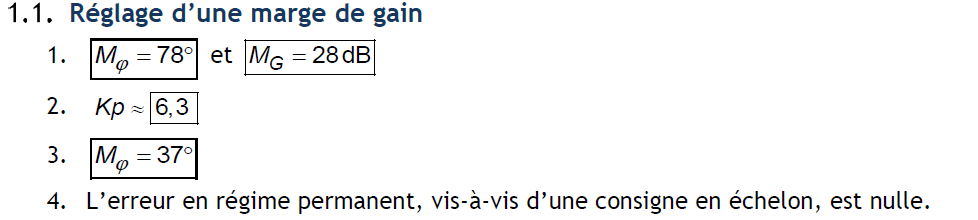
\includegraphics[width=.65\linewidth]{cor_01}
%%\textit{}
%\end{center}

\ifprof
\else
\begin{center}
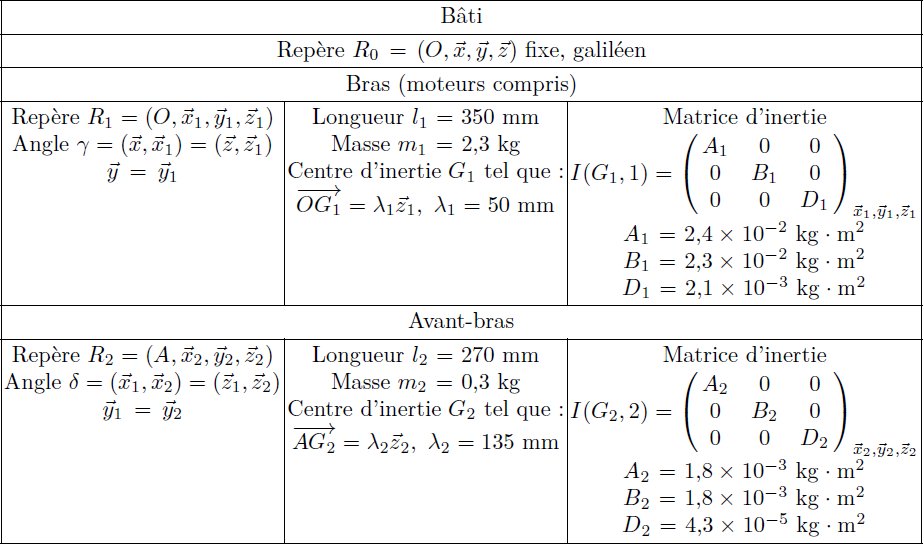
\includegraphics[width=.8\linewidth]{fig_06}
%\textit{}
\end{center}

\begin{center}
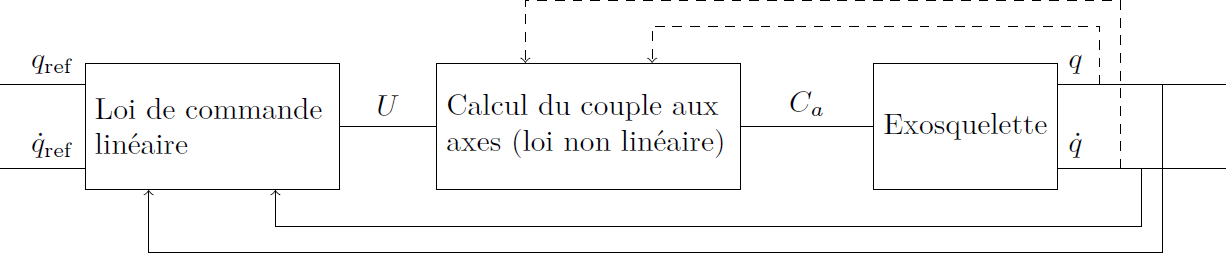
\includegraphics[height=\linewidth]{fig_07}
%\textit{}
\end{center}
\fi

\ifprof
\else
\begin{marginfigure}[-3cm]
\centering

\includegraphics[width=3cm]{Cy_03_01_TD_PI_07_Hexapode_qr}
\end{marginfigure}
\fi
